\FloatBarrier\section{Procedural Scene Generation}
\label{sec:procedural}
\label{sec:simulator}
% The first stage of \housionna{} constructs the agricultural environment in Houdini. A parameterised node network generates geometry, assigns material attributes, and places gateways, sensor nodes, and measurement surfaces for the ray-tracing stage. It can represent alternative crop layouts or infrastructure configurations without manually rebuilding every scene.


The first stage of  \housionna{}  constructs the agricultural environment in Houdini 22, a proprietary procedural modelling tool (the free non-commercial edition suffices) in which each scene is the output of a node network rather than a manually edited model. Exposed parameters control crop species, growth stage, plant spacing, room size, infrastructure, occupancy, and device density. The network generates the geometry and assigns material attributes per primitive (material, thickness, and water content), so these properties can vary within one scene. Measurement surfaces for radio maps are added the same way. Scene generation is deterministic: random choices use explicit seeds, so a scene is fully defined by its parameter values and can be regenerated exactly from them. Batches are organised with Houdini’s Procedural Dependency Graph (PDG), which turns combinations of parameter values into work items, each producing one scene variant (\cref{sec:execution}). Alternative crop layouts and infrastructure configurations therefore do not have to be rebuilt by hand, and every result can be traced back to the parameters that generated its scene.





% \subsection{Agricultural Geometry}\label{sec:geometry}
% The scene parameters include plant spacing, canopy height and depth, leaf orientations, infrastructure layout, and device positions; gateways and sensor nodes can be placed anywhere, including on plants and on mobile robots. Plants are generated with L-systems in three growth stages, optionally with fruit, so growth is represented by a sequence of static scenes. People, autonomous robots, windows, and metal frames can be added as disturbances of the channel. A geometric growth parameter is not automatically a validated physiological model. \Cref{fig:growth_stages} illustrates the three growth stages. \gilles{be sure to mention where these models are coming from.}






\subsection{Agricultural Geometry}\label{sec:geometry}
Plants are generated with L-systems, using Houdini's L-system operator. Species-specific rules, written for this work and included in the repository~\cite{housionna}, produce five growth stages (0--4) per species, optionally with fruit. Growth is therefore represented by a sequence of static scenes; the stages are geometric snapshots, not a validated physiological growth model. \Cref{fig:growth_stages} shows the five growth stages of cherry tomato. Leaves are single surfaces rather than closed volumes, and their slab thickness is a material attribute (\cref{sec:materials}), so paths through them are not lost to the \SI{1}{cm} segment limit (\cref{sec:solver}). Plants are placed on trays at a set spacing, in a room of parametric size with its structural frame, windows, sprayers, and secondary structure. People and robots are added as disturbances of the channel; an occupancy parameter and a seed set their number and positions.

Gateways and sensor nodes are points carrying their role, transmit power, antenna pattern, polarisation, and orientation. Each sensor node is attached to its plant at a seeded position, at a clearance of \SI{2}{cm} from leaves, stems, and trays, and stays attached through the growth stages. Like a physical sensor, it moves with the plant, and its orientation follows the main stem, so the antenna axis and polarisation change as the plant grows. Gateways are distributed evenly over a horizontal plane above the crop at a set density per floor area, with at least one, and face downwards. Devices can also be mounted on robots or people as mobile nodes.
   
% \begin{figure*}[htp]
% \centering
% \newcommand{\gridimg}[2]{%
%   \begin{minipage}[t]{0.19\linewidth}\raggedright
%     \includegraphics[width=\linewidth]{figures/procedural/#1_#2}\\
%     {\scriptsize x=#1\\y=#2\par}
%   \end{minipage}}%
% \newcommand{\gridrow}[1]{%
%   \gridimg{0}{#1}\hfill\gridimg{1}{#1}\hfill\gridimg{2}{#1}\hfill\gridimg{3}{#1}\hfill\gridimg{4}{#1}\par\smallskip}%
% \gridrow{0}
% \gridrow{1}
% \gridrow{2}
% \caption{Procedural scene variations.}
% \label{fig:procedural_matrix}
% \end{figure*}



% \begin{figure*}[htp]
% \centering
% \newcommand{\gridimg}[2]{%
%   \begin{minipage}[t]{0.19\linewidth}\raggedright
%     \includegraphics[width=\linewidth]{figures/procedural/#1_#2}\\
%     {\scriptsize sensors=#1\\y=#2\par}
%   \end{minipage}}%
% \newcommand{\gridrow}[1]{%
%   \gridimg{0}{#1}\hfill\gridimg{1}{#1}\hfill\gridimg{2}{#1}\hfill\gridimg{3}{#1}\hfill\gridimg{4}{#1}\par\smallskip}%
% \gridrow{0}
% \gridrow{1}
% \gridrow{2}
% \caption{Procedural scene variations.}
% \label{fig:procedural_matrix}
% \end{figure*}


% \begin{figure}[ht]
% \centering
% \newcommand{\stageimg}[1]{%
%   \begin{minipage}[t]{0.32\linewidth}\raggedright
%     \includegraphics[width=\linewidth]{figures/growth_stage/#1}\\[-1pt]
%     {\scriptsize #1\par}
%   \end{minipage}}%
% \stageimg{seedling}\hfill\stageimg{vegetative}\hfill\stageimg{mature}
% \caption{Plant growth stages.}
% \label{fig:growth_stages}
% \end{figure}



% testing

% \begin{figure}[ht]
% \centering
% \stageimg{ocimum_basilicum_v1_gen1}{Gen.~1}\hfill\stageimg{ocimum_basilicum_v1_gen2}{Gen.~2}\hfill\stageimg{ocimum_basilicum_v1_gen3}{Gen.~3}
% \caption{\textit{Ocimum basilicum}, variant 1.}
% \label{fig:ocimum_v1}
% \end{figure}

% \begin{figure}[ht]
% \centering
% \stageimg{ocimum_basilicum_v2_gen1}{Gen.~1}\hfill\stageimg{ocimum_basilicum_v2_gen2}{Gen.~2}\hfill\stageimg{ocimum_basilicum_v2_gen3}{Gen.~3}
% \caption{\textit{Ocimum basilicum}, variant 2.}
% \label{fig:ocimum_v2}
% \end{figure}

% \begin{figure}[ht]
% \centering
% \stageimg{ocimum_basilicum_v3_gen1}{Gen.~1}\hfill\stageimg{ocimum_basilicum_v3_gen2}{Gen.~2}\hfill\stageimg{ocimum_basilicum_v3_gen3}{Gen.~3}
% \caption{\textit{Ocimum basilicum}, variant 3.}
% \label{fig:ocimum_v3}
% \end{figure}

% \newcommand{\stageimg}[2]{%
%   \begin{minipage}[t]{0.32\linewidth}\raggedright
%     \includegraphics[width=\linewidth]{figures/growth_stage/#1}\\[-1pt]
%     {\scriptsize #2\par}
%   \end{minipage}}

% \begin{figure}[t]
% \centering
% \stageimg{fragaria_x_ananassa_v1_gen1}{Gen.~1}\hfill\stageimg{fragaria_x_ananassa_v1_gen2}{Gen.~2}\hfill\stageimg{fragaria_x_ananassa_v1_gen3}{Gen.~3}\\[2pt]
% \stageimg{solanum_lycopersicum_v1_gen1}{Gen.~1}\hfill\stageimg{solanum_lycopersicum_v1_gen2}{Gen.~2}\hfill\stageimg{solanum_lycopersicum_v1_gen3}{Gen.~3}
% \caption{Three generated growth stages of strawberry (\textit{Fragaria $\times$ ananassa}, top) and tomato (\textit{Solanum lycopersicum}, bottom).}
% \label{fig:growth_stages}
% \end{figure}





\newcommand{\stageimg}[2]{%
  \begin{minipage}[t]{0.31\linewidth}\raggedright
    \includegraphics[width=\linewidth]{figures/growth_stage/#1}\\[-1pt]
    {\scriptsize #2\par}
  \end{minipage}}

% \begin{figure}[ht]
% \centering
% \stageimg{fragaria_x_ananassa_v1_gen1}{Gen.~1}\hfill\stageimg{fragaria_x_ananassa_v1_gen2}{Gen.~2}\hfill\stageimg{fragaria_x_ananassa_v1_gen3}{Gen.~3}\\[2pt]
% \stageimg{solanum_lycopersicum_v1_gen1}{Gen.~1}\hfill\stageimg{solanum_lycopersicum_v1_gen2}{Gen.~2}\hfill\stageimg{solanum_lycopersicum_v1_gen3}{Gen.~3}
% \caption{Three generated growth stages of strawberry (\textit{Fragaria $\times$ ananassa}, top) and tomato (\textit{Solanum lycopersicum}, bottom).}\label{fig:growth_stages}
% \end{figure}




\begin{figure}[hbtp]
    \centering
    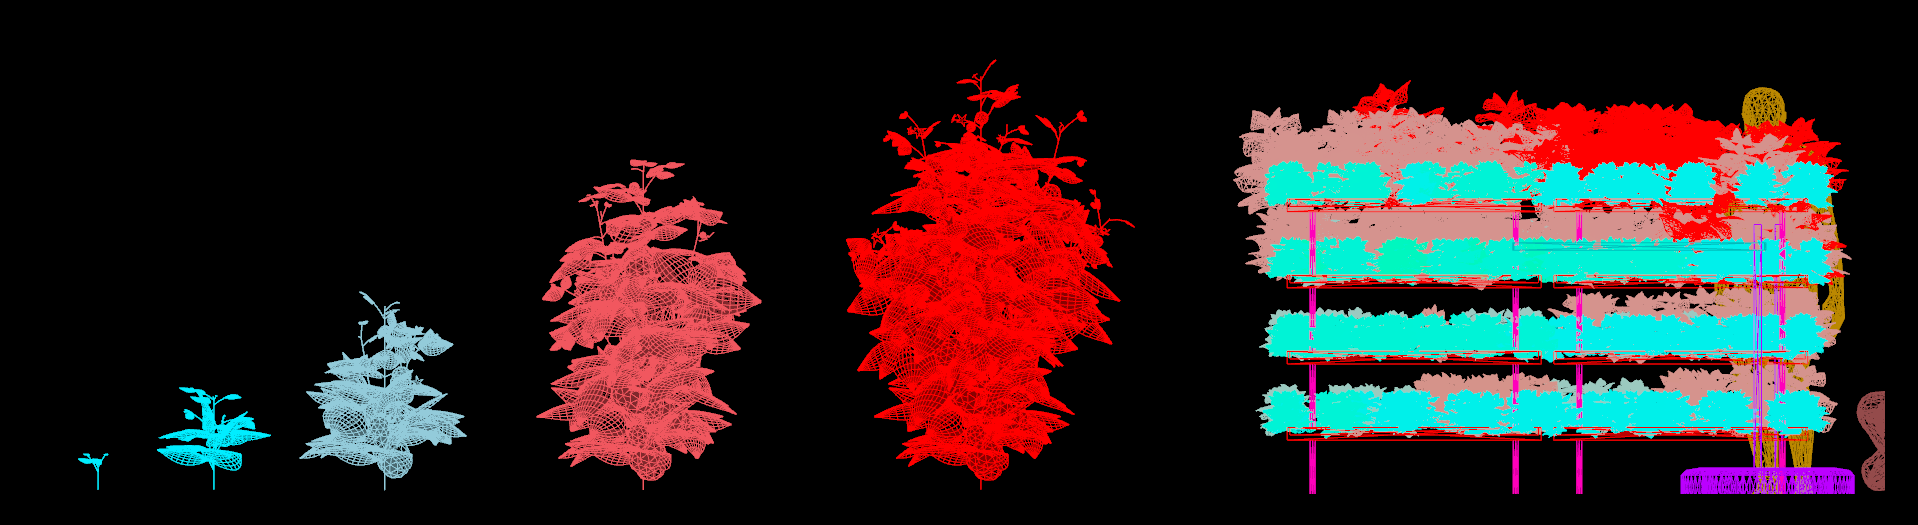
\includegraphics[width=0.98\linewidth]{figures/screenshots/combined5.png}%
    % 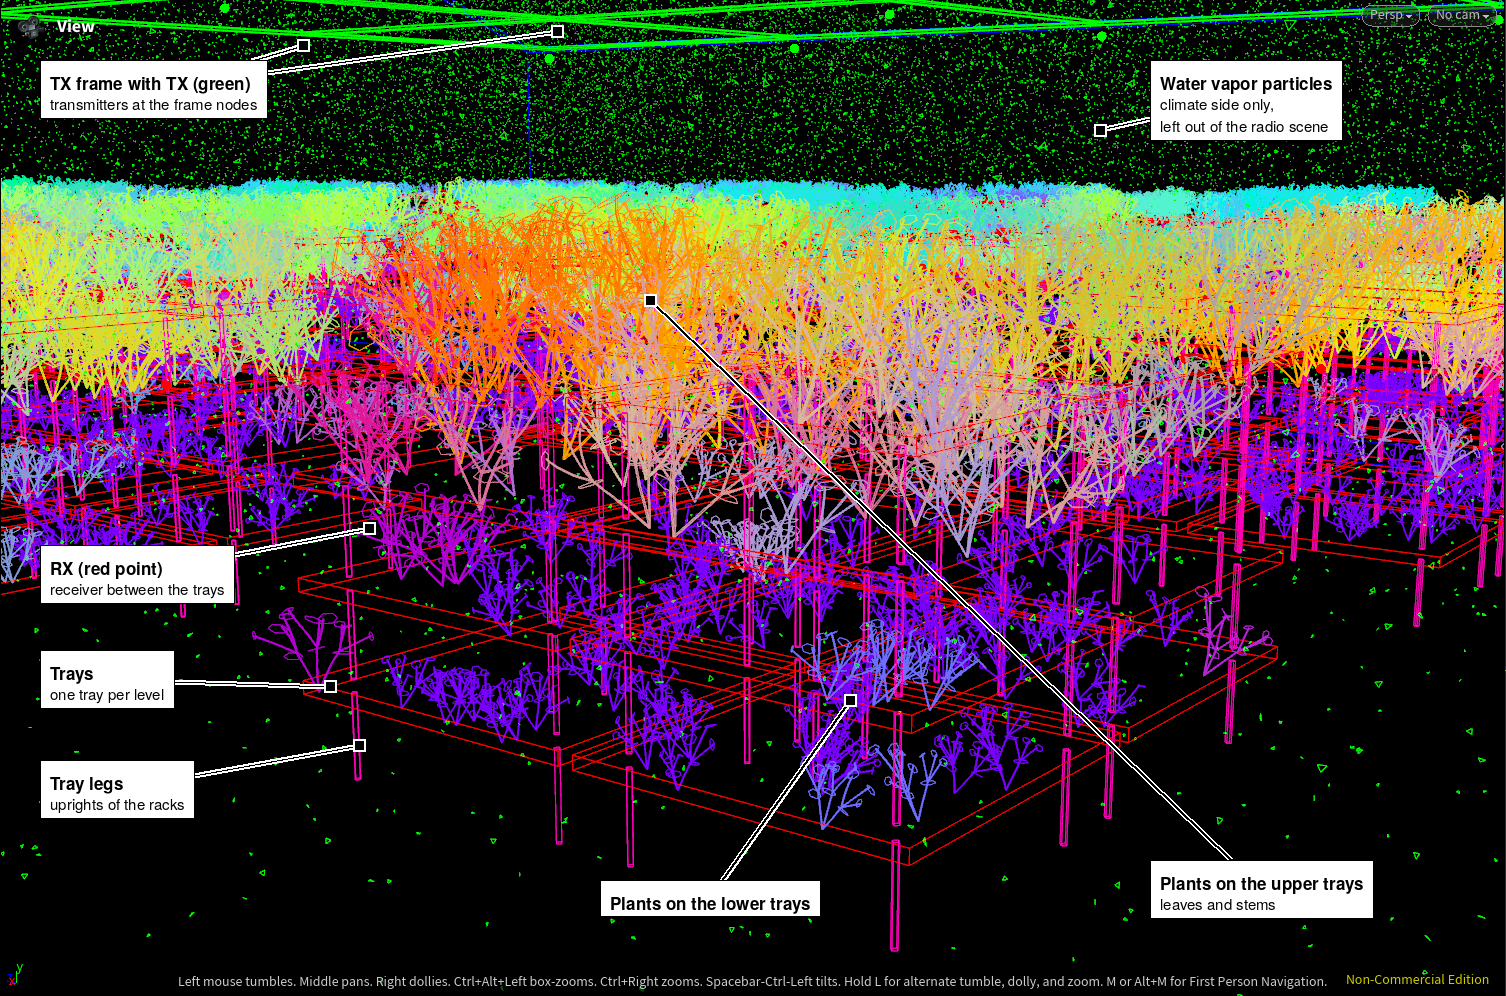
\includegraphics[width=0.5\linewidth]{figures/procedural/annotated_00bbc1c9.png}
    \caption{Five generated growth stages and one rack of cherry tomato (\textit{Solanum lycopersicum}).}\label{fig:growth_stages}
\end{figure}




% \subsection{Radio Materials}\label{sec:materials}
% The built-in ITU-R P.2040 materials of Sionna are bounded in frequency~\cite{itu2040}: apart from wood and glass, they are defined only from \SI{1}{GHz}, which excludes the \SI{868}{MHz} and \SI{915}{MHz} bands. \housionna{} therefore adds frequency-dependent models and records a source and status for each material: Cole--Cole fits of common building materials measured from \SIrange{0.2}{67}{GHz}~\cite{zhekov2020}, conductors for metal structures, water and nutrient solution~\cite{liebe1991}, soils~\cite{itu527}, and the dual-dispersion vegetation model for leaves and stems~\cite{ulaby1987}. The vegetation coefficients are not yet verified, and fruit and growing media use placeholder values, so plant materials must be treated as provisional. ITU-R P.833 provides an independent vegetation-attenuation reference for appropriate scenarios~\cite{itu833}; it does not replace calibration for the specific crop and geometry.


\subsection{Radio Materials}\label{sec:materials}
The built-in ITU-R P.2040 materials of Sionna are bounded in frequency~\cite{itu2040}: apart from wood and glass, they are defined only from \SI{1}{GHz}, which excludes the \SI{868}{MHz} and \SI{915}{MHz} bands. \housionna{} therefore adds frequency-dependent models and records a source, status, and valid frequency range for each material, with a warning when a run extrapolates beyond that range. The models are Cole--Cole fits of common building materials measured from \SIrange{0.2}{67}{GHz}~\cite{zhekov2020}, conductors for metal structures, water and nutrient solution~\cite{liebe1991}, soils~\cite{itu527}, the dual-dispersion vegetation model for leaves~\cite{ulaby1987}, and a four-term Cole--Cole model of dry skin for people~\cite{gabriel1996}. Material properties are evaluated at the frequency of each run or work item. Material, slab thickness, and water content are primitive attributes, so water content (\% of fresh mass for leaves, default \SI{80}{\percent}; \% of volume for soils) can vary within a scene and across work items. Leaves use an assumed slab thickness of \SI{0.3}{mm}. The vegetation model is not validated for the crops considered here, and fruit and growing media use placeholder values, so plant materials must be treated as provisional. ITU-R P.833 provides an independent vegetation-attenuation reference for appropriate scenarios~\cite{itu833}; it does not replace calibration for the specific crop and geometry.
